\section{Generalisation}\label{sec:generalisation}
\textbf{Frozen Non-Learned gates generalise poorly:} We trained both ReLU and GaLU networks on standard MNIST dataset to close to $100\%$ accuracy. We observed that the GaLU network trains a bit faster than the ReLU network (see \Cref{fig:galu-relu} ). However, the test performances were around $96\%$ and  $98\%$ for GaLU and ReLU networks respectively\footnote{In the case of GaLU, in order to eliminate the effect of initialisation, we trained with identical as well as independent initialisation for the gating as well as the main network in the GaLU. }. We trained ReLU and GaLU networks on standard CIFAR-10 dataset close to $100\%$ training accuracy. In this case, the test performances were around $64\%$ and $72\%$ for GaLU and ReLU networks respectively. 
\begin{comment}
Note that, in the case of $\N(\Tg_{\dagger},\infty;\Tv_t)$, we were initialising $\Tg_0\in \R^{d_{net}}$ and $\Tv_0\in \R^{d_{net}}$ in a statistically independent manner. Thus, in order to eliminate the effect of the initialisation, we also compared DGNs of the form  $\N(\Theta_t,\infty;\Theta_t)$ and $\N(\Tv_{\dagger},\infty;\Tv_t)$ (which we call as frozen ReLU networks). We trained both ReLU and frozen ReLU networks on standard MNIST dataset to close to $100\%$ accuracy. The test performances were around $96\%$ and  $98\%$ for frozen ReLU and ReLU networks respectively. We trained ReLU and GaLU networks on standard CIFAR-10 dataset close to $100\%$ training accuracy. In this case, the test performances were around $72\%$ and $64\%$ for ReLU and frozen ReLU networks respectively.
\end{comment}


\textbf{Frozen Learned gates generalise better:} In the case of MNIST, 
In the case of CIFAR-10, GaLU with learned gates achieved a test performance of $70\%$ (which is better than GaLU with non-learned gates with a performance of  $64\%$).


\begin{figure*}
\resizebox{\textwidth}{!}{
\begin{tabular}{ccc}
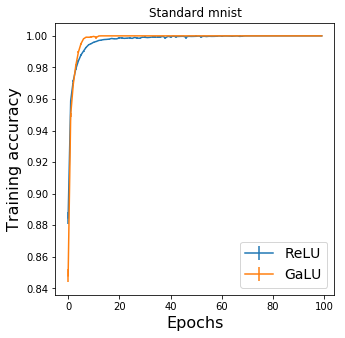
\includegraphics[scale=0.1]{figs/mnist-normal-opt.png}
&
%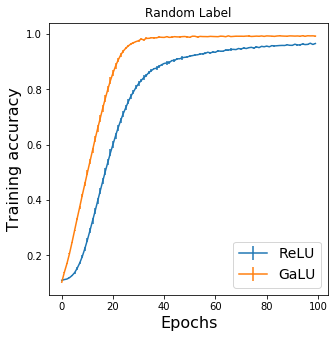
\includegraphics[scale=0.1]{figs/mnist-rand-label.png}
%&
%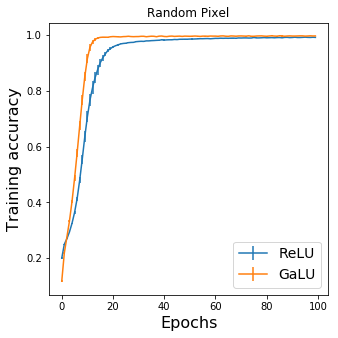
\includegraphics[scale=0.1]{figs/mnist-rand-pixel.png}
%&
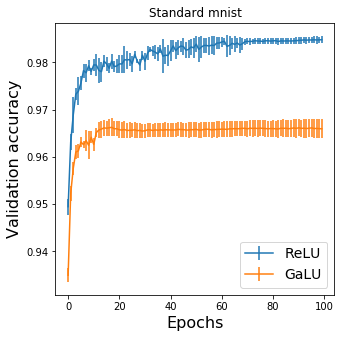
\includegraphics[scale=0.1]{figs/mnist-normal-gen.png}
&
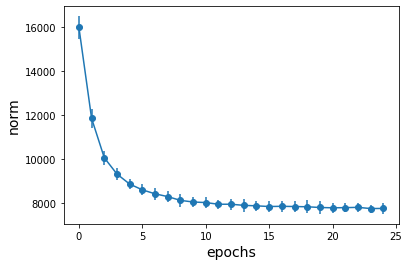
\includegraphics[scale=0.125]{figs/path-gram.png}
	\end{tabular}
}
\caption{First two plots from the left show optimisation and generalisation in ReLU and GaLU networks for standard MNIST. The right most plot shows $\nu_t=y^\top (\widehat{M}_t)^{-1}y$, where $M_t=\Phi_t^\top \Phi_t$.}
\label{fig:galu-relu}
\end{figure*}


\textbf{NPK dynamics in ReLU:} We consider ``Binary''-MNIST data set with two classes namely digits $4$ and $7$, with the labels taking values in $\{-1,+1\}$ and squared loss. We trained a standard DNN with ReLU activation ($w=100$, $d=5$). Recall from \Cref{sec:intro}, that $M_t=\Phi^\top_t\Phi_t$  (the Gram matrix of the features) and let $\widehat{M}_t=\frac{1}{trace(M_t)}M_t$ be its normalised counterpart. For a subset size, $n'=200$ ($100$ examples per class) we plot $\nu_t=y^\top (\widehat{M}_t)^{-1} y$, (where $y\in\{-1,1\}^{200}$ is the labeling function), and observe that $\nu_t$ reduces as training proceeds (see middle plot in \Cref{fig:path-norm}). Note that $\nu_t=\sum_{i=1}^{n'}(u_{i,t}^\top y)^2 (\hat{\rho}_{i,t})^{-1}$, where $u_{i,t}\in \R^{n'}$ are the orthonormal eigenvectors of $\widehat{M}_t$ and $\hat{\rho}_{i,t},i\in[n']$ are the corresponding eigenvalues. Since $\sum_{i=1}^{n'}\hat{\rho}_{i,t}=1$, the only way $\nu_t$ reduces is when more and more energy gets concentrated on $\hat{\rho}_{i,t}$s for which $(u_{i,t}^\top y)^2$s are also high. However, in $M_t=(x^\top x)\odot \lambda_t$, only $\lambda_t$ changes with time. Thus, $\lambda_t(s,s')$ which is a measure of overlap of sub-networks active for input examples $s,s'\in[n]$, changes in a manner to reduce $\nu_t$. We can thus infer that the \emph{right} active sub-networks are learned over the course of training.
\begin{comment}
\begin{figure}
\centering
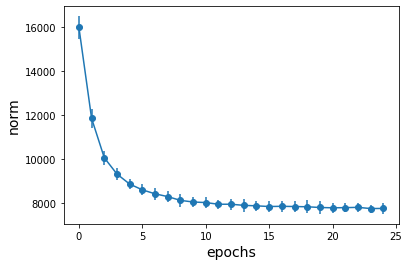
\includegraphics[scale=0.5]{figs/path-gram.png}
\caption{Shows $\nu_t=y^\top (\widehat{M}_t)^{-1}y$, where $M_t=\Phi_t^\top \Phi_t$.}
\label{fig:path-norm}
\end{figure}
\end{comment}

\begin{comment}
\FloatBarrier
\begin{table}[h]
\centering
\resizebox{\columnwidth}{!}{
\begin{tabular}{|c|c|c|}\hline
Terminology& Notation & Remarks\\\hline
ReLU & $\N(\Theta_t,\infty;\Theta_t)$ & $\Theta_t\in \R^{d_{net}}$\\\hline
GaLU (Frozen) &$\N(\Tg_{\dagger},\infty;\Tv_t)$ & $\Tv_t\in \R^{d_{net}}$, $\Tg_{\dagger}\in \R^{d_{net}}$\\\hline
Soft-ReLU &$\N(\Theta_t,\beta;\Theta_t)$ & $G\in(0,1)$ (not decoupled)\\\hline
Soft-GaLU &$\N(\Tg_t,\beta;\Tv_t)$ &  $G\in(0,1)$ (decoupled) \\\hline
\end{tabular}
}
\caption{Shows the variants of DGNs in the experiments. Here, $\dagger$ stands for frozen weights that are initialised by not trained.}% In all our experiments (expect one) we set $\epsilon=0$ in $\chi_{\epsilon}$.}
\label{tb:dgn-family}
\end{table}
\end{comment}

\begin{comment}
\begin{figure*}
\resizebox{\textwidth}{!}{
\begin{tabular}{cccc}
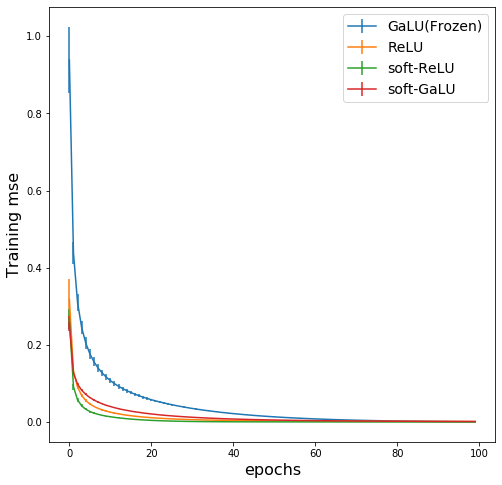
\includegraphics[scale=0.1]{figs/allnet-train.png}
&
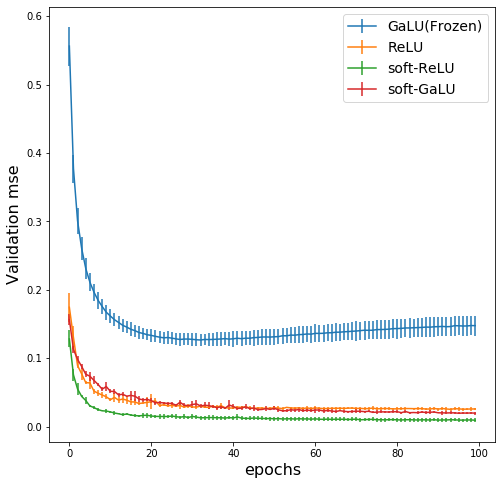
\includegraphics[scale=0.1]{figs/allnet-gen.png}
&
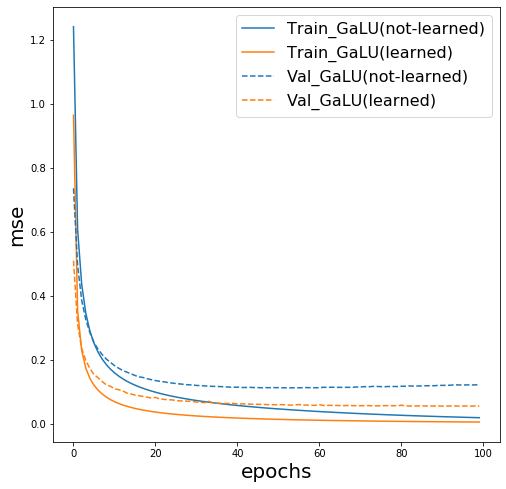
\includegraphics[scale=0.1]{figs/galu-learn-no-learn.png}
&
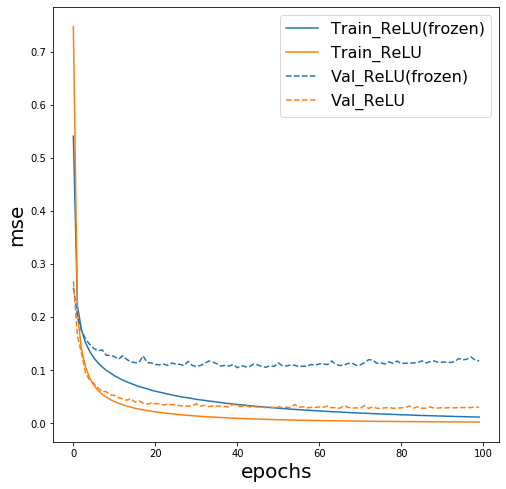
\includegraphics[scale=0.1]{figs/relu-froze-no-froze.png}

\end{tabular}
}
\caption{The left two plots show respectively the training and generalisation in the $4$ different networks with $w=100$, $d=6$. Generalisation performance (dotted lines) of learned gates vs unlearned gates ($3^{rd}$ from left), adaptable gates vs frozen gates (rightmost). The plots are averaged over $5$ runs. }
\label{fig:adapt}
\end{figure*}

\begin{figure*}
\resizebox{\textwidth}{!}{
\begin{tabular}{ccccc}
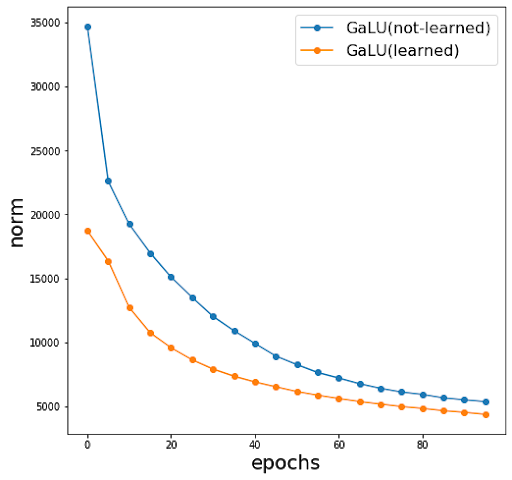
\includegraphics[scale=0.1]{figs/galu-learn-no-learn-knorm.png}
&
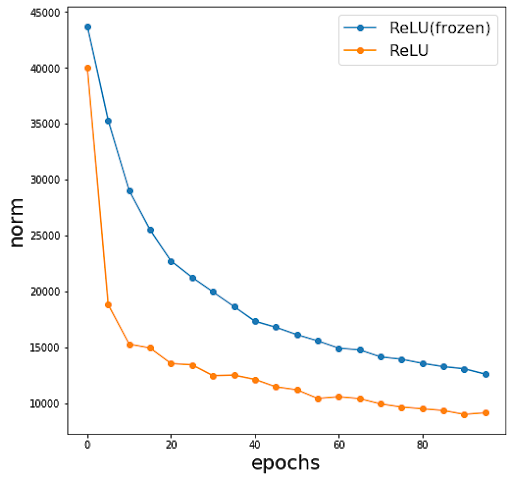
\includegraphics[scale=0.1]{figs/relu-froze-no-froze-knorm.png}
&
%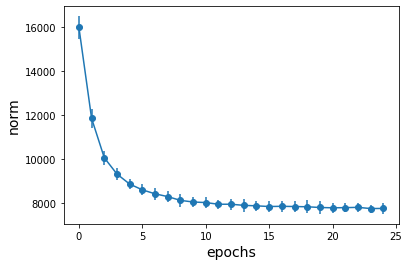
\includegraphics[scale=0.18]{figs/path-gram.png}

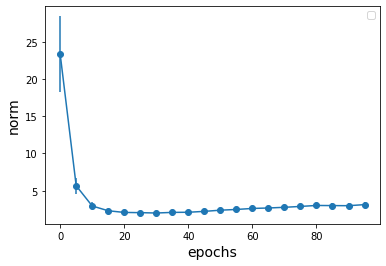
\includegraphics[scale=0.18]{figs/activation-gram-unnorm.png}
&
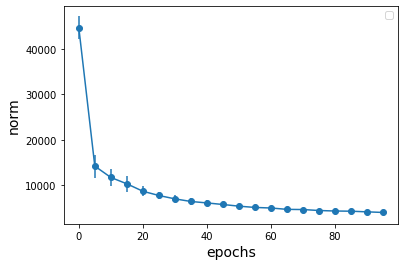
\includegraphics[scale=0.18]{figs/activation-gram-norm.png}
\end{tabular}
}
\caption{Shows $\nu_t=y^\top (H_t)^{-1}y$ for (from the left) i) $H_t=\widehat{K}_t$, ii) $H_t=\widehat{K}_t$,  (iii) $H_t=K^a_t$ (iv) $H_t=\widehat{K^a_t}$. Here $K^a_t$ is the Gram matrix of activations in the soft-GaLU network.}
\label{fig:adapt-norm}
\end{figure*}
\end{comment}
\begin{comment}

We now explain the idea behind the various gates (and some more) in \Cref{tb:dgn-family} as follows:

$1.$ The most general gate is called the \emph{soft-GaLU} gate denoted by $\N(\Tg,\beta;\Tv)$. Here, the gating values and hence the path activation levels are decided by $\Tg_t\in\R^{d_{net}}$, and the path strengths are decided by $\Tv_t\in \R^{d_{net}}$. This network has $2d_{net}$ parameters. % Both $\Tg_0$ and $\Tv_0$ are independent of each other and initialised according to Assumption~\ref{assmp:mainone}.

$2.$ The standard DNN with ReLU gating is denoted by $\N(\Theta_t,\infty;\Theta_t)$, where $\infty$ signifies that the outputs are $0/1$ (see \Cref{tb:dgn-parameterised}). Here, both the gating (and hence path activation levels) and the path strengths are decided by the same parameter namely $\Theta_t\in\R^{d_{net}}$.

$3.$ $\N(\Theta_t,\beta;\Theta_t)$ is a DNN with what we call the \emph{soft-ReLU} gates, where the gating values are in $(0,1+\epsilon)$ instead of $0/1$. Here too, like the standard ReLU networks, both the gating values and the path strengths are decided by $\Theta_t\in\R^{d_{net}}$.

$4.$ $\N(\Tg_{\dagger}, \infty;\Tv_t)$ is what we call a GaLU-frozen DGN, where the gating parameters $\Tg\in \R^{d_{net}}$ are initialised but not trained. 

$5.$ $\N(\Tg_t,\beta;\Tv_{\dagger})$ is a network where only the gating parameters $\Tg_t\in \R^{d_{net}}$ are trainable and the parameters which dictate the path strengths namely $\Tv$ are initialised by not trained.

\end{comment}

\subsection{Feature Learning: Preliminary analysis }
\begin{comment}
 \textbf{Hard gate/ReLU artefact:} 
%We refer to the function $\chi_\epsilon(v)$ in \Cref{tb:dgn-parameterised} as the \emph{soft} gating function.
The NTF matrix has two components given by $\Psi_t(m,s)={\phi_{x_s,\G_t }^\top\frac{\partial w_{t}} {\partial \theta(m)}+ \frac{\partial \phi_{x_s,\G_t }^\top}{\partial \theta(m)} w_{t}}$. In the case of ReLU activation, the gating values are either $0/1$, the activation levels are also $0/1$ and hence their derivative is $0$. Thus, in the case of standard DNN with ReLU activations the change in the gating pattern with respect to time (captured by $\frac{\partial \phi_{x_s,\G_t }^\top}{\partial \theta(m)} w_{t}$) is unaccounted for both in analysis as well as in the gradient descent update rule, i.e., when a gradient step is taken, it is not known beforehand the effect of the gradient step on the gating pattern. 

%In contrast, the `soft-gating' is differentiable, and hence if follows that $\frac{\partial \phi_{x_s,\G_t }^\top}{\partial \theta(m)} w_{t}\neq 0$, which is also accounted in the analysis.
 \textbf{Soft-Gating}: We refer to the function $\chi_\epsilon(v)$ in \Cref{tb:dgn-parameterised} as the \emph{soft} gating function, which takes values in $(0,1+\epsilon)$.  An important feature of the soft-gate is that, the term $\frac{\partial \phi_{x_s,\G_t }^\top}{\partial \theta(m)} w_{t}\neq 0$, which is accounted in both analysis as well as the gradient descent update rule.
 
 
\textbf{Gram Matrices with gate adaptation term:} In the case of $\N(\Tg_t,\beta;\Tv_t)$ networks (which we call as soft-GaLU networks), since there are two set of parameters (total $2d_{net}$) $\Psi_t^\top=[{\Psi^w}^\top_t,{\Psi^a}^\top_t]$ is a $n\times 2d_{net}$, we have $K_t=K^w_t+K^a_t$,  where $K^w_t={\Psi^w_t}^\top \Psi^w_t$, and $K^a_t={\Psi^a_t}^\top \Psi^a_t$. In the case of $\N(\Theta_t,\beta;\Theta_t)$ (which we call as soft-ReLU)  we have $K_t={K^w_t}+{K^a_t}+{\Psi^w_t}^\top {\Psi^a_t}+{\Psi^a_t}^\top {\Psi^w_t}$.

\begin{definition} 
For a soft-GaLU DGN, using any $i\in[d_{in}]$, define $\delta(s,s')\stackrel{def}= \underset{{p\rsa i}}{\sum} \sum_{m=1}^{d_{net}}\frac{\partial A_{\Tg_0}(x_s,p)}{\partial \tg(m)} \frac{\partial A_{\Tg_0}(x_{s'},p)}{\partial \tg(m)}$.
\end{definition}

\begin{lemma} Under Assumptions~\ref{assmp:mainone},~\ref{assmp:maintwo}, in soft-GaLU networks we have: (i) $\E{K_0}=\E{K^w_0}+\E{K^a_0}$, 
 (ii) $\E{K^w_0}=\sigma^{2(d-1)} (x^\top x)\odot \lambda$,  (iii) $\E{K^a_0}=\sigma^{2d}  (x^\top x)\odot \delta$
\end{lemma}
\end{comment}
Recall that $\G_t\stackrel{def}=\{G_{x_{s},t}(l,i) \in [0,1], \forall s\in[n],l\in[d-1],i\in[w]\}$. We now define the following:

$\bullet$ \textbf{Active Gates:} For an input $x_{s}\in \R^{d_{in}}$, and a threshold value $\tau_{\A}\in (0,1+\epsilon)$, define $\G_t^{\A}(x_s,\tau_{\A})\stackrel{def}=\left\{G_{x_s,t}(l,i)\colon G_{x_s,t}(l,i)> \tau_{\A}, l\in[d-1],i\in[w]\right\}$. These are the gates that are \emph{on} (i.e., more than threshold $\tau_{\A}$) for input $x_s\in\R^{d_{in}}$.

$\bullet$ \textbf{Sensitive Gates:} For an input $x_{s}\in \R^{d_{in}}$, and a threshold value $\tau_{\S}>0$, define $\G_{t}^{\S}(x_s,\tau_{\S})\stackrel{def}=\cup_{m=1}^{d_{net}}\left\{G_{x_s,t}(l,i)\colon \left|\frac{\partial G_{x_s,t}(l,i)}{\partial \tg(m)}\right| >\tau_{\S},l\in[d-1],i\in[w] \right\}$. These are set of gates that are sensitive to changes in anyone of the $\tg(m),m\in[d_{net}]$ tunable parameters that control the gates.

$\bullet$ \textbf{Relation between sensitive and active gates:} From the nature of the soft-gating function $\chi_{\epsilon}(v)$ it follows that for any given $\tau_{\A}\in(0,1+\epsilon)$, it follows that $\G_t^{\A}(x_s,\tau_{\A})\cap \G_t^{\S}(x_s,\tau_{\S})=\emptyset,\forall \tau_{\S}>\frac{d \chi_{\epsilon}(v)}{d v}|_{v=\chi^{-1}_{\epsilon}(\tau_{\A})}$. Also, note that as $\tau_{\A}\ra (1+\epsilon)$, $\tau_{\S}\ra 0$.

$\bullet$ \textbf{Sensitivity of Activations:} For a path $p$, and a gating parameter $\tg(m),m\in[d_{net}]$ we have $\frac{\partial A_{\Tg_t}(x_s,p)}{\partial \tg(m)}$ to be equal to
\begin{align}\label{eq:sensitivity}
\sum_{l=1}^{d-1} \Big(\frac{\partial G_{x_s,\Tg_t}(l,p(l))}{\partial \tg(m)} \Big)\Big(\Pi_{l'\neq l} G_{x_s,\Tg_t}(l',p(l'))\Big)
\end{align}

In what follows we assume that $\tau_{\S}>\frac{d \chi_{\epsilon}(v)}{d v}|_{v=\chi^{-1}_{\epsilon}(\tau_{\A})}$.

$\bullet$ \textbf{Active Sub-Network:} Which paths are active for input $x_s\in\R^{d_{in}}$?\quad Choose a threshold $\tau_{\A}$ close to $1$. The paths that pass through gates in $\G_t^{\A}(x_s,\tau_{\A})$ do not matter much in gate adaptation because they are already \emph{on}, and are responsible for holding the memory for input $x_s\in\R^{d_{in}}$. In particular, \eqref{eq:sensitivity} evaluates close to $0$ for such paths because $\left|\frac{\partial G_{x_s,\Tg_t}(l,p(l))}{\partial \tg(m)}\right|<\frac{d \chi_{\epsilon}(v)}{d v}|_{v=\chi^{-1}_{\epsilon}(\tau_{\A})}$.

$\bullet$ \textbf{Sensitive Sub-Network:} Which paths are learning for input $x_s\in\R^{d_{in}}$? \quad Those paths that have one gate from $\G^{\S}_t(x_s,\tau_{\S})$ and the rest of the $(d-2)$ gates from the set  $\G^{\A}_t(x_s,\tau_{\A})$. For such paths, the magnitude of at least one of the $(d-1)$ terms in \eqref{eq:sensitivity} will be greater than $\tau_{\S}(\tau_{A})^{(d-2)}$, and the rest of the $(d-2)$ terms will contain a term whose magnitude is less than $\frac{d \chi_{\epsilon}(v)}{d v}|_{v=\chi^{-1}_{\epsilon}(\tau_{\A})}$ component and hence will contribute less to the summation.

$\bullet$ \textbf{Role of $\beta$} for now is limited to an analytical convenience, especially to address the non-differentiability artefact in ReLU gates. The ideas is that as $\beta\ra\infty$, the analysis applies more sharply to networks with ReLU gates.
